% Chapter 1
%\chapter{مقدمه}

\section{مقدمه}

سیستم‌های متمرکز تا پیش از این بیشتر نیازها را برطرف می‌کردند، اما در دنیای امروزی و با افزایش تعداد دستگاه‌های متصل، چالش‌های جدیدی مطرح شده است. هزینه‌های بالای ناشی از انتقال حجم زیاد داده‌ها از یک جهت، و افزایش نگرانی‌ها درباره امنیت اطلاعات حساس و شخصی از جهت دیگر، محققان را به سمت استفاده از الگوریتم‌های غیرمتمرکز و توزیع‌شده در حوزه یادگیری ماشین سوق داده است. یکی از جدیدترین زیرمجموعه‌های مهم و پرکاربرد روش‌های یادگیری توزیع‌شده، یادگیری فدرال است که بسیار مورد توجه قرار گرفته است.


در روش یادگیری فدرال، برخلاف رویکردهای متمرکز یادگیری ماشین، تجزیه و تحلیل داده‌ها به دستگاه‌های لبه%
\LTRfootnote{Edge Devices}
یا کاربران%
\LTRfootnote{Clients}
منتقل می‌شوند
\cite{ma2022state}.
این روش، به عنوان یک جایگزین مطلوب برای مدل‌سازی داده‌ها در محیط‌هایی با تعداد زیادی کاربر معرفی شده است. در این چارچوب، به‌جای انتقال داده‌های اصلی، پارامترهای مدل‌های محلی در هر مرحله از فرآیند آموزش به سمت سرور منتقل می‌شوند، که این امر زمینه‌ساز بهبود امنیت و کاهش هزینه‌های ارتباطی می‌باشد.
در شکل
\ref{federated_learning}
این معماری به نمایش گذاشته شده است.

\begin{figure}[t]
	\centering
	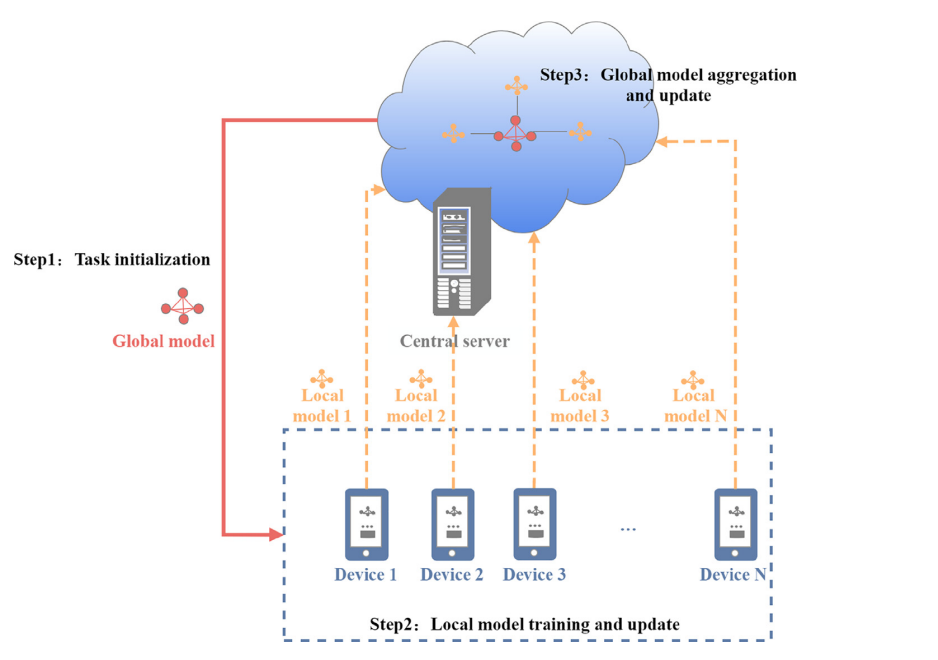
\includegraphics[scale=0.595]{images/chap1/federated_learning.png}%
	\caption{%
		یادگیری فدرال 
		\cite{ma2022state}%
		.
	}
	\label{federated_learning}
	\centering
\end{figure}

سرور در حقیقت نقش رهبری را ایفا می‌کند و با توجه به نوع داده‌ها، یک مدل شبکه عصبی%
\LTRfootnote{Neural Network}
ایجاد کرده و آن را به سمت کاربران ارسال می‌کند. در ادامه کاربران با توجه به داده‌های خود شبکه را آموزش می‌دهند و بعد از چند بار تکرار به‌صورت محلی، وزن‌های به‌روزرسانی شده را به سمت سرور بر می‌گردانند. همان‌طور که در شکل
\ref{federated_learning}
مشاهده می‌شود، داده‌ها همگی در سمت کاربران قرار گرفته‌اند و به سمت سرور ارسال نمی‌شوند. عدم اجبار در به اشتراک گذاشتن اطلاعات گره‌ها در یادگیری فدرال، کمک شایانی به حفظ حریم شخصی کاربران می‌کند
\cite{smith2017federated}.



یکی از روش‌های اصلی و پرکاربرد در یادگیری فدرال روش میانگین‌گیری فدرال یا
\lr{FedAvg}
است که توسط محققان گوگل در سال 2017 معرفی شد
\cite{mcmahan2017communication}.
این الگوریتم به منظور بهینه‌سازی مدل‌های یادگیری ماشین در یک محیط توزیع‌شده طراحی شده است. در این روش داده‌ها به‌صورت محلی در دستگاه‌های کاربران باقی می‌مانند و تنها به‌روزرسانی‌های مدل به اشتراک گذاشته می‌شوند. رویکرد اصلی
\lr{FedAvg}
بر مبنای ترکیب به‌روزرسانی‌های محلی از دستگاه‌های مختلف به یک مدل سراسری استوار است.


یکی از مزایای اصلی
\lr{FedAvg}
این است که به‌طور موثری با چالش ناهمگنی داده‌ها مقابله می‌کند.
میانگین‌گیری وزنی در
\lr{FedAvg}
به مدل کمک می‌کند تا به‌روزرسانی‌های مختلف را به گونه‌ای ترکیب کند که این ناهمگنی‌ها را در نظر بگیرد. به عبارت دیگر، اگر یک دستگاه داده‌های بیشتری داشته باشد، تأثیر بیشتری بر مدل نهایی خواهد داشت. این رویکرد باعث می‌شود که مدل فدرال به تعادل بهتری در یادگیری از داده‌های ناهمگن برسد و کارایی بالاتری داشته باشد. این ویژگی به ویژه در کاربردهایی مانند فروشگاه برنامه‌های کاربردی که کاربران متنوع و داده‌های متفاوتی دارند، بسیار سودمند است و می‌تواند به بهبود عملکرد مدل در شرایط واقعی کمک شایانی کند.






\section{کارهای مرتبط}

\subsection{
	روش جابه‌جایی فدرال%
	\LTRfootnote{Federated Swapping}
	\lr{\texttt{\fontspec{Times New Roman} (FedSwap)}}
}
در این روش، یک عملیات جدید به نام جابه‌جایی فدرال یا
\lr{FedSwap}
پیشنهاد شده است که به عنوان جایگزینی برای برخی از دوره‌های
\lr{FedAvg}
در یادگیری فدرال به کار می‌رود.
این عملیات با هدف بهبود فرآیند یادگیری فدرال و کاهش تاثیرات منفی داده‌های
\lr{non-IID}
طراحی شده است
\cite{chiu2020semisupervised}.


در روش‌ یادگیری فدرال، پس از هر تکرار، مدل‌های محلی از دستگاه‌های نهایی جمع‌آوری شده و یک مدل جامع از ترکیب آن‌ها ساخته می‌شود. اما در روش
\lr{FedSwap}%
، به‌جای این که این ادغام در هر تکرار انجام شود، سرور مدل‌های محلی را در گام‌های مشخصی بین دستگاه‌ها جابه‌جا می‌کند. در واقع، در انتهای برخی مراحل، عملیات جابه‌جایی و در انتهای برخی دیگر، ادغام مدل‌ها صورت می‌گیرد. این مراحل بر اساس پارامترهایی که به عنوان ورودی تعریف می‌شوند، تعیین می‌گردند.
جهت درک بهتر این ساختار به شکل
\ref{federated_swapping}
توجه نمایید.


\begin{figure}[t]
	\centering
	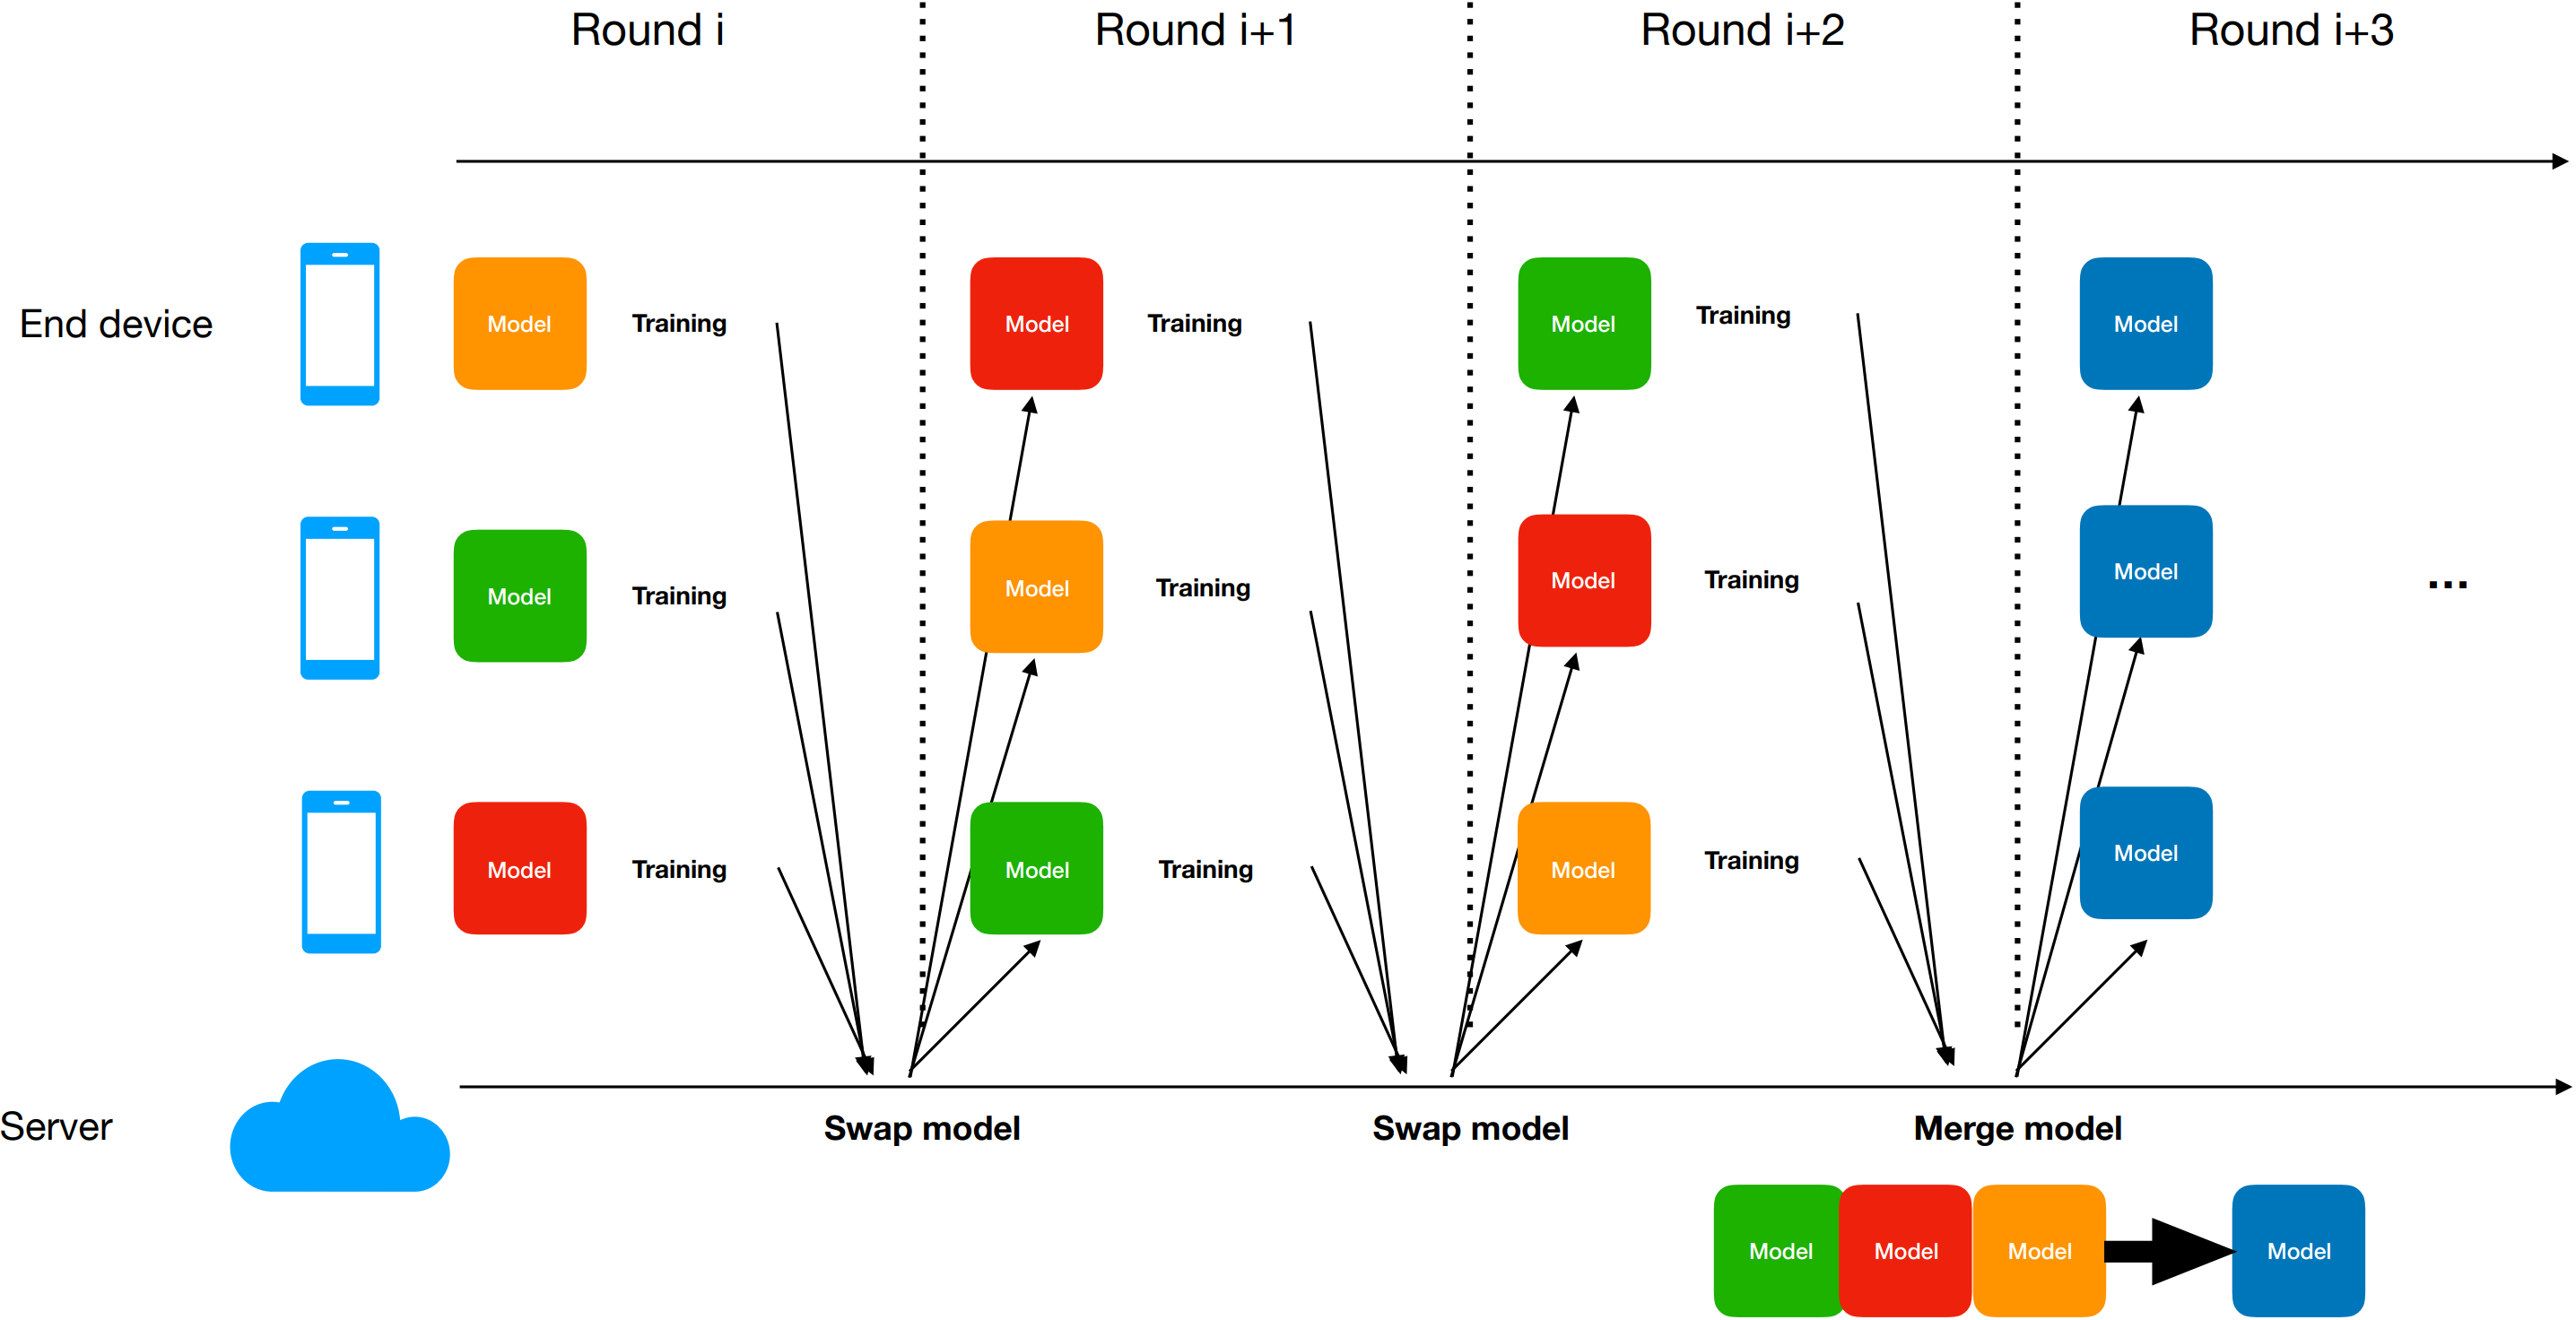
\includegraphics[scale=0.179]{images/chap4/federated_swapping.png}%
	\caption{%
		روش جابه‌جایی فدرال
		\cite{chiu2020semisupervised}%
		.
	}
	\label{federated_swapping}
	\centering
\end{figure}








\subsection{معیارهای مشابهت}

 فرض کنید \( X \) ماتریسی با ابعاد \( n \times p_1 \) باشد که \( X \in \mathbb{R}^{n \times p_1} \) شامل \( n \) نمونه و \( p_1 \) ویژگی است. همچنین، \( Y \) ماتریسی با ابعاد \( n \times p_2 \) باشد که \( Y \in \mathbb{R}^{n \times p_2} \) شامل \( n \) نمونه و \( p_2 \) ویژگی است. فرض می‌شود که \( p_1 \) کمتر یا مساوی \( p_2 \) است.
 
 
 هدف طراحی و تحلیل یک شاخص شباهت عددی \( s(X, Y) \) است که بتواند بازنمایی‌های%
 \LTRfootnote{Representations}
 موجود در ماتریس‌های \( X \) و \( Y \) را هم درون یک شبکه عصبی و هم بین شبکه‌های عصبی مختلف مقایسه کند. چنین شاخصی به درک بهتر تأثیر عوامل مختلف در یادگیری عمیق کمک می‌کند.
 
 به عنوان مثال، در بررسی شبکه‌های عصبی، ماتریس \( X \) می‌تواند نمایانگر فعال‌سازهای%
 \LTRfootnote{Activations}
 نورون‌ها در یک لایه خاص برای \( n \) نمونه ورودی باشد و ماتریس \( Y \) می‌تواند نمایانگر فعال‌سازهای نورون‌ها در لایه‌ای دیگر یا حتی در یک شبکه عصبی دیگر برای همان \( n \) نمونه باشد. مقایسه این دو ماتریس اطلاعات مهمی درباره نحوه یادگیری و بازنمایی داده‌ها توسط شبکه عصبی ارائه می‌دهد.
 
 
 در این بخش به بررسی روش‌های مختلفی که برای سنجش مشابهت بین بازنمایی‌های شبکه‌های عصبی استفاده می‌شود، پرداخته خواهد شد. یکی از روش‌های مهم در این زمینه استفاده از پایه‌های متعامد است. به‌طور خاص، فرض می‌شود که \( Q_X \) و \( Q_Y \) پایه‌های متعامدی برای ستون‌های ماتریس‌های \( X \) و \( Y \) هستند. به این معنا که \( Q_X \) و \( Q_Y \) به‌صورت \( Q_X = X(X^T X)^{-1/2} \) و \( Q_Y = Y(Y^T Y)^{-1/2} \) تعریف شده‌اند. این پایه‌های متعامد امکان تحلیل مؤثرتر بازنمایی‌های شبکه عصبی و سنجش دقیق‌تر شباهت‌های آن‌ها را فراهم می‌کنند.
 تمامی رابطه‌های مورد استفاده در بخش
 \ref{sec_similarity_measurement_criteria}%
 ، از مرجع 
 \cite{kornblith2019similarity} 
 برگرفته شده‌اند.
 
 
 
 
 \subsection{
 	قرینه مجموع اختلاف مطلق%
 	\LTRfootnote{Opposite Sum of Absolute Difference}
 	\lr{\texttt{\fontspec{Times New Roman} (OSAD)}}
 }
 معیار سنجش شباهت  
 \lr{OSAD}  
 برای مقایسه ماتریس‌هایی با ساختار یکسان و ابعاد ثابت استفاده می‌شود. اگر ابعاد ماتریس‌ها \( n \times p \) باشد، شباهت از طریق رابطه زیر اندازه‌گیری می‌شود:  
 \[
 OSAD = -\sum_{i=1}^n \sum_{j=1}^{p_1} Z_{ij}  
 \quad \text { where } \quad  
 Z = |X-Y|  
 \]  
 
 در این رابطه، \( X \) و \( Y \) ماتریس‌های ورودی و \( Z \) ماتریس اختلاف مطلق بین آن‌ها است. در نهایت، قرینه مجموع مقادیر \( Z \) به‌عنوان معیار  
 \lr{OSAD}  
 استفاده می‌شود.  
 
 با فرض ثابت و یکسان بودن ابعاد و مقدارهای اولیه ماتریس‌ها،  
 \lr{OSAD}  
 یک ابزار ساده و قابل اعتماد برای مقایسه و ارزیابی شباهت بین دو ماتریس محسوب می‌شود و اختلاف‌ها را به‌طور مؤثری محاسبه می‌کند.
 
  
 
 \subsection{
 	تحلیل همبستگی کانونی%
 	\LTRfootnote{Canonical Correlation Analysis}
 	\lr{\texttt{\fontspec{Times New Roman} (CCA)}}
 }
 تحلیل همبستگی کانونی یا  
 \lr{CCA}  
 با هدف شناسایی ترکیب‌هایی از ویژگی‌ها در دو مجموعه داده مختلف انجام می‌شود تا بیشترین همبستگی بین آن‌ها پیدا شود. به عنوان مثال، در یک مجموعه داده، اطلاعات قد و وزن و در دیگری، اطلاعات سن و درآمد افراد قرار دارد.  
 
 ابتدا، داده‌ها استاندارد می‌شوند و سپس  
 \lr{CCA}  
 بردارهای وزنی را محاسبه می‌کند تا ترکیب‌هایی از ویژگی‌ها ایجاد شوند که حداکثر همبستگی را داشته باشند. هدف این است که ترکیبی از ویژگی‌های یک مجموعه با ترکیبی از ویژگی‌های مجموعه دیگر، بالاترین ارتباط را داشته باشد.  
 
 \lr{CCA}  
 به دنبال یافتن پایه‌هایی برای دو ماتریس است که همبستگی بین داده‌ها به حداکثر برسد. ضریب همبستگی کانونی  
 \(\rho_i\)  
 به صورت زیر تعریف می‌شود:  
 \[
 \rho_i = \max_{\mathbf{w}_X^i, \mathbf{w}_Y^i} \text{corr}(X \mathbf{w}_X^i, Y \mathbf{w}_Y^i)
 \]  
 برای اطمینان از استقلال ترکیب‌ها، باید شرط‌های زیر برقرار باشند:  
 \[
 \begin{array}{ll}
 	\forall_{j<i} & X \mathbf{w}_X^i \perp X \mathbf{w}_X^j \\
 	\forall_{j<i} & Y \mathbf{w}_Y^i \perp Y \mathbf{w}_Y^j
 \end{array}
 \]  
 
 همچنین، برای ارزیابی شباهت دو شبکه عصبی، از معیار  
 \( R^2_{CCA} \)  
 استفاده می‌شود که میزان توضیح‌دهندگی ترکیب‌های خطی را اندازه‌گیری می‌کند.  
 \[
 R^2_{CCA} = \frac{\sum_{i=1}^{p1} \rho^2_i}{p1} = \frac{||Q^T_Y Q_X||^2_F}{p1}
 \]  
 
 در نهایت،  
 \lr{CCA}  
 به شناسایی ترکیب‌های خطی از ویژگی‌ها کمک می‌کند تا روابط پنهان بین دو مجموعه داده مشخص شوند. 
 
 
 
 
 
 \subsection{
 	معیار استقلال هیلبرت-اشمیت%
 	\LTRfootnote{Hilbert-Schmidt Independence Criterion}
 	\lr{\texttt{\fontspec{Times New Roman} (HSIC)}}
 }
 برای بررسی وابستگی و شباهت بین دو مجموعه داده، از معیار  
 \lr{HSIC}  
 استفاده می‌شود که به‌طور خاص برای اندازه‌گیری همبستگی طراحی شده است. این معیار، برای داده‌های مرکزیت‌یافته \( X \) و \( Y \)، به‌صورت زیر تعریف می‌شود:  
 \[
 \frac{1}{(n - 1)^2} \text{tr}(XX^TYY^T) = ||\text{cov}(X^T, Y^T)||_F^2
 \]  
 
 معیار  
 \lr{HSIC}  
 این رابطه را با استفاده از توابع هسته‌ای تعمیم می‌دهد تا وابستگی بین ماتریس‌های داده را بررسی کند. عناصر \( K_{ij} \) و \( L_{ij} \) از طریق توابع هسته‌ای \( k(x_i, x_j) \) و \( l(y_i, y_j) \) محاسبه می‌شوند  
 \cite{gretton2005measuring}.  
 
 تعریف  
 \lr{HSIC}  
 به‌صورت زیر است:  
 \[
 \text{HSIC}(K, L) = \frac{1}{(n - 1)^2} \text{tr}(KHLH)
 \]  
 که در آن \( H \) ماتریس مرکزیت‌دهنده است و به‌صورت  
 \( H_n = I_n - \frac{1}{n} 11^T \)  
 تعریف می‌شود.  
 
 اگر توابع هسته‌ای خطی باشند،  
 \lr{HSIC}  
 به همان رابطه اولیه برمی‌گردد. این معیار، ارزیابی دقیق و قابل اعتمادی از وابستگی بین داده‌ها فراهم می‌کند و به درک بهتر ساختارهای پیچیده کمک می‌کند.
 
 
 
 
 
 \subsection{
 	هم‌ترازی هسته مرکزی%
 	\LTRfootnote{Centered Kernel Alignment}
 	\lr{\texttt{\fontspec{Times New Roman} (CKA)}}
 }
 معیار  
 \lr{HSIC}  
 نسبت به مقیاس‌بندی یکسان ویژگی‌ها ناپایدار است و ممکن است در تغییر مقیاس‌ها، نتایج نادرستی ارائه دهد. برای حل این مشکل، از شاخص نرمال‌شده‌ای به نام هم‌ترازی هسته مرکزی یا  
 \lr{CKA}  
 استفاده می‌شود  
 \cite{cortes2012algorithms, cristianini2001kernel}.  
 
 رابطه  
 \lr{CKA}  
 به شکل زیر تعریف می‌شود:  
 \[
 \text{CKA}(K, L) = \frac{\text{HSIC}(K, L)}{\sqrt{\text{HSIC}(K, K) \cdot \text{HSIC}(L, L)}}  
 \]  
 که در آن صورت کسر همان  
 \lr{HSIC}  
 اصلی بوده و مخرج کسر برای نرمال‌سازی و حذف تأثیر مقیاس‌بندی استفاده می‌شود. این نرمال‌سازی باعث می‌شود نتیجه مستقل از مقیاس‌بندی باشد و شباهت‌های واقعی را بهتر نمایش دهد.  
 
 استفاده از  
 \lr{CKA}  
 به‌ویژه در تحلیل بازنمایی‌های شبکه‌های عصبی مؤثرتر از  
 \lr{HSIC}  
 است، زیرا علاوه بر سنجش دقیق‌تر شباهت‌ها، در برابر تغییرات مقیاس‌بندی نیز مقاوم است. بنابراین،  
 \lr{CKA}  
 ابزاری قدرتمند برای درک و تحلیل بازنمایی‌های مختلف در یادگیری عمیق محسوب می‌شود.
 
 
 
 \subsection{
 	هم‌ترازی هسته مرکزی بدون مداخله%
 	\LTRfootnote{Deconfounded Centered Kernel Alignment}
 	\lr{\texttt{\fontspec{Times New Roman} (dCKA)}}
 }\label{sec_dCKA}
 فرض کنید \(X\) یک مجموعه داده با \(n\) نمونه و \(p\) ویژگی باشد. نمایش لایه‌های \(m_1\) و \(m_2\) از دو شبکه عصبی \(f_1\) و \(f_2\) به‌صورت  
 \(X^{m_1}_{f_1}\)  
 و  
 \(X^{m_2}_{f_2}\)  
 است  
 \cite{cui2022deconfounded}.  
 
 شباهت هر جفت نمونه در این لایه‌ها با معیار شباهت \( k(\cdot, \cdot) \) محاسبه شده و در ماتریس‌های  
 \(K^{m_1}_{f_1}\)  
 و  
 \(K^{m_2}_{f_2}\)  
 نشان داده می‌شود:  
 \[
 K^{m_1}_{f_1} = k(X^{m_1}_{f_1}, X^{m_1}_{f_1}), \quad K^{m_2}_{f_2} = k(X^{m_2}_{f_2}, X^{m_2}_{f_2})  
 \]  
 سپس، برای مقایسه دو ماتریس از معیار شباهت \( s(\cdot, \cdot) \) استفاده می‌شود:  
 \[
 s^{m_1,m_2}_{f_1,f_2} = s(K^{m_1}_{f_1}, K^{m_2}_{f_2})  
 \]  
 
 در روش  
 \lr{CKA}  
 شباهت بین دو ماتریس، میزان شباهت بین دو شبکه عصبی را نشان می‌دهد. اما این ماتریس‌ها تحت تأثیر شباهت اولیه داده‌ها  
 \( K^0 \)  
 قرار دارند که ممکن است نتایج نادرستی ایجاد کند. برای حل این مشکل، شباهت ورودی  
 \( K^0 \)  
 از ماتریس‌ها حذف می‌شود تا تنها عملکرد شبکه‌ها سنجیده شود. این روش به حذف مداخله‌گر معروف است  
 \cite{cui2022deconfounded}.  
 
 حذف شباهت اولیه به‌صورت زیر انجام می‌شود:  
 \[
 dK^{m_1}_{f_1} = K^{m_1}_{f_1} - \hat{\alpha}^{m_1}_{f_1} K^0,  \quad dK^{m_2}_{f_2} = K^{m_2}_{f_2} - \hat{\alpha}^{m_2}_{f_2} K^0  
 \]  
 که در آن، ضرایب \(\hat{\alpha}\) برای حداقل‌کردن اندازه ماتریس‌های اصلاح‌شده تعیین می‌شوند. این فرآیند باعث می‌شود اثر شباهت اولیه حذف شده و مقایسه به‌طور دقیق‌تر انجام گیرد.  
 
 در نهایت، شباهت‌های جدید با معیار  
 \( s(\cdot, \cdot) \)  
 سنجیده می‌شوند:  
 \[
 ds^{m_1,m_2}_{f_1,f_2} = s(dK^{m_1}_{f_1}, dK^{m_2}_{f_2})  
 \]  
 این روش امکان ارزیابی معتبر شباهت‌های بازنمایی را بدون تأثیر متغیرهای مداخله‌گر فراهم می‌کند.
 
 
 
 
 
 
 \subsection{شاخص مشابهت بین شبکه‌های عصبی}
 برای مقایسه کامل دو شبکه عصبی، لازم است که تمامی لایه‌ها به‌طور جداگانه ارزیابی و سپس یک شاخص شباهت کلی ارائه شود. ابتدا، شباهت هر لایه با استفاده از معیارهای شباهت محاسبه و سپس این معیارها میانگین‌گیری می‌شوند تا نمای کلی از شباهت بین دو شبکه به دست آید.
 
 در لایه‌های  
 \lr{Fully Connected}  
 ساختار لایه‌ها به‌صورت ماتریس‌های دوبعدی است و مقایسه به‌راحتی انجام می‌شود. اما در لایه‌های  
 \lr{Convolutional}  
 که چندبعدی هستند، ابتدا این لایه‌ها با  
 \lr{Flattening}  
 به دو بعد تبدیل می‌شوند تا امکان مقایسه فراهم شود. 
 این شاخص شباهت به فهم بهتر ساختار شبکه‌ها و تصمیم‌گیری در مورد بهبود مدل‌ها کمک می‌کند.
  
 
 
 
 
\section{مدل سیستم}

\subsection{
		جابه‌جایی فدرال برپایه شباهت%
		\LTRfootnote{Similarity-based Federated Swapping}
		\lr{\texttt{\fontspec{Times New Roman} (SimFedSwap)}}%
}


هدف اصلی این پژوهش، انتخاب و جابه‌جایی دستگاه‌های نهایی براساس شباهت مدل‌های شبکه عصبی است. برای این منظور، ابتدا باید مدل‌ها با یکدیگر مقایسه شوند تا میزان شباهت آن‌ها تعیین گردد. در روش پیشنهادی 
\lr{SimFedSwap}، 
مدلی که کمترین شباهت را با مدل دستگاه فعلی دارد برای جابه‌جایی انتخاب می‌شود، زیرا شباهت زیاد بین مدل‌ها باعث کاهش اثربخشی جابه‌جایی خواهد شد.

جابه‌جایی مدل‌ها بین دستگاه‌هایی با داده‌های متفاوت، تنوع در داده‌ها و بهبود فرآیند یادگیری را به‌همراه دارد. این تنوع موجب می‌شود مدل‌ها سریع‌تر همگرا شده و عملکرد کلی افزایش یابد. همچنین، این رویکرد به مقابله بهتر با چالش‌های داده‌های 
\lr{non-IID} 
کمک می‌کند.

در این روش، تمامی مدل‌های شبکه عصبی ابتدا به سرور ارسال شده و سپس سرور شباهت آن‌ها را بررسی و جابه‌جایی را مدیریت می‌کند. این کار با فرض محدودیت دستگاه‌های نهایی در سخت‌افزار و منابع انجام می‌شود. عملیات پردازشی و تصمیم‌گیری به‌طور کامل بر روی سرور انجام شده و دستگاه‌های نهایی تنها به تبادل داده‌ها و به‌روزرسانی‌های سبک می‌پردازند.





\subsection{تاثیرات جابه‌جایی}

در این بخش، تاثیرات مختلف جابه‌جایی مدل‌ها بر ترافیک شبکه و حریم شخصی بررسی شده است. ابتدا نشان داده می‌شود که روش‌های جابه‌جایی مدل‌ها هزینه ترافیک شبکه را نسبت به روش‌های سنتی افزایش نمی‌دهند و در برخی موارد حتی به کاهش آن کمک می‌کنند. سپس به بررسی تاثیرات این جابه‌جایی‌ها بر حریم شخصی کاربران پرداخته می‌شود که در آن خطرات مرتبط با تبادل مدل‌ها بین کاربران، با واسطه یا بدون واسطه سرور ارزیابی می‌شود.

\subsubsection{تاثیرات جابه‌جایی مدل‌ها بر ترافیک شبکه}
در این بخش نشان داده می‌شود که جابه‌جایی مدل‌ها در روش‌های  
\lr{FedSwap}  
و  
\lr{SimFedSwap}  
هیچ هزینه اضافی در ترافیک شبکه نسبت به  
\lr{FedAvg}  
ایجاد نمی‌کنند و حتی می‌توانند ترافیک را بهبود بخشند.

در روش  
\lr{FedAvg}،  
مدل‌ها در هر گام  
\( h_1 \times h_2 \)  
به سرور ارسال شده و پس از میانگین‌گیری بازگردانده می‌شوند، که هزینه هر گام برابر با  
\( 2Ks \)  
است. در مقابل، در روش  
\lr{FedSwap}،  
مدل‌ها در \( h_2 - 1 \) مرحله بین کاربران مبادله می‌شوند و تنها در گام آخر به سرور ارسال می‌گردند. هزینه این مبادله  
\( Ks \)  
است.

در روش  
\lr{SimFedSwap}،  
مدل‌ها در هر گام به سرور ارسال و بازگردانده می‌شوند، که هزینه هر گام  
\( 2Ks \)  
خواهد بود.

کاهش هزینه‌های ارتباطی این روش‌ها نسبت به  
\lr{FedAvg}  
به‌صورت زیر محاسبه می‌شود:  
\[
\frac{FedAvg - FedSwap}{FedAvg} = \frac{2h_1h_2 - h_2 - 1}{2h_1h_2},  
\quad  
\frac{FedAvg - SimFedSwap}{FedAvg} = \frac{h_1 - 1}{h_1}  
\]  

با پارامترهای \(h_1 = 5\) و \(h_2 = 3\)، روش  
\lr{FedSwap}  
۸۶٫۶۶ درصد و  
\lr{SimFedSwap}  
۸۰ درصد هزینه‌های شبکه را کاهش می‌دهند  
(شکل \ref{compare_swap_net_traffic}).


\subsubsection{تأثیر جابه‌جایی مدل‌ها بر حریم شخصی}
در روش  
\lr{FedAvg}،  
پس از آموزش محلی، مدل‌ها به سرور ارسال و سپس تجمیع می‌شوند. در این روش، ارتباط مستقیم بین کاربران وجود ندارد و تنها تعاملات با سرور انجام می‌شود که این امر به حفظ حریم شخصی کمک می‌کند. کاربران فقط به سرور اعتماد می‌کنند و نیازی به اعتماد متقابل میان آن‌ها نیست.
اما در روش‌های جابه‌جایی مدل‌ها، چه با واسطه سرور و چه بدون واسطه، خطرات مربوط به حریم شخصی افزایش می‌یابد.

استفاده از روش  
\lr{Differential Privacy}  
در جابه‌جایی مدل‌ها با واسطه‌گری سرور، امکان مدیریت بهتر نویز اضافه‌شده را فراهم می‌کند، ولی همچنان نیاز به اعتماد به سرور وجود دارد. در حالی که در جابه‌جایی مستقیم مدل‌ها بدون واسطه، کاربران باید خودشان نویز لازم را به مدل‌ها اضافه کنند که این کار پیچیدگی بیشتری به همراه دارد و احتمال افشای اطلاعات را افزایش می‌دهد.

به‌طور کلی، استفاده از سرور به‌عنوان واسطه به حفظ بهتر حریم شخصی کمک می‌کند، اما جابه‌جایی مستقیم مدل‌ها میان کاربران به تدابیر امنیتی بیشتری نیاز دارد.





\subsection{نحوه جابه‌جایی}
زمانی که همه مدل‌های شبکه عصبی در سرور مرکزی قرار دارند، وظیفه سرور این است که تصمیم بگیرد کدام کاربران مدل‌های خود را با یکدیگر جابه‌جا کنند. برای انجام این کار، ابتدا باید مدل‌ها با یکدیگر مقایسه شوند تا میزان شباهت بین آن‌ها مشخص شود. سپس، بر اساس این شباهت‌ها تعیین می‌شود که کدام کاربران مدل‌های شبکه عصبی خود را با یکدیگر مبادله کنند، یا به عبارت دیگر، سرور مشخص می‌کند کدام مدل به کدام کاربر ارسال شود.

\subsubsection{جابه‌جایی حریصانه}

در روش حریصانه، از بین تمام کاربران موجود، یک کاربر به‌صورت تصادفی انتخاب می‌شود. سپس مدل شبکه عصبی این کاربر با مدل‌های تمامی کاربران دیگر مقایسه می‌شود تا میزان شباهت آن‌ها سنجیده شود. در این مرحله، کاربری که مدل شبکه عصبی او کمترین شباهت را با مدل کاربر انتخاب‌ شده دارد، به عنوان کاربر مقصد برای جابه‌جایی مدل انتخاب می‌شود. پس از این انتخاب، سرور مدل‌های این دو کاربر را با یکدیگر جابه‌جا می‌کند و در نهایت این دو کاربر را از لیست انتخاب حذف خواهد کرد.

پس از انجام این جابه‌جایی، فرایند مشابهی برای کاربران باقی‌مانده تکرار می‌شود. ابتدا یک کاربر دیگر به‌صورت تصادفی انتخاب می‌شود و دقیقا همان روند بالا برای آن تکرار خواهد شد.
شبه کد کامل این روش در الگوریتم
\ref{algo_greedy_swapping}
ارائه شده است. علاوه بر این، نمادهای مختص به این الگوریتم در جدول
\ref{tabel_GreedySwappingNotations}
و همچنین تمامی نمادهای پایه در جدول
\ref{tabel_FedAvgNotations}
توضیح داده شده‌اند.
هدف از این جداول، فراهم کردن درکی جامع از نحوه عملکرد و پیاده‌سازی الگوریتم می‌باشد.


\begin{LTR}
	\SetAlgoNlRelativeSize{-1}
	\begin{algorithm}[t]
		\begin{RTL}
			\caption{%
				جابه‌جایی حریصانه
				\lr{(Greedy Swapping)}
			}
			\label{algo_greedy_swapping}
		\end{RTL}
		
		\begin{latin}
			\SetKwFunction{GreedySwapping}{GreedySwapping}
			\SetKwProg{Fn}{Function}{:}{end}
			\Fn{\GreedySwapping{}}{
				$LRS$ = copy of $U_t$\;
				$NS$ = (length of $U_t$ // 2) * $SP$\;
				\BlankLine
				
				\For{$NS$ times}{
					$RandomIndex$ = random integer between $0$ and length of $LRS$\;
					$SCB = LRS[RandomIndex]$\;
					remove $SCB$ from $LRS$\;
					
					\BlankLine
					Initialize $LstSimilarity$ as an empty list\;
					\For{each $RC \in LRS$}{
						$Sim = \texttt{ModelSimilarity} (w^{SCB}, w^{RC})$\;
						Append $Sim$ to $LstSimilarity$\;
					}
					$MinSimilarityIndex$ = index of the minimum value in $LstSimilarity$\;
					$SCD = LRS[MinSimilarityIndex]$\;
					remove $SCD$ from $LRS$\;
					\BlankLine
					
					$\texttt{Swap}(SCB, SCD)$\;
				}
			}
		\end{latin}
	\end{algorithm}
\end{LTR}

\begin{table}[h]
	\centering
	\caption{نمادهای مختص الگوریتم جابه‌جایی حریصانه}
	\label{tabel_GreedySwappingNotations}
	\begin{tabular}{cr}
		\hline
		متغیر & توضیحات \\
		\hline
		$LRS \, (LstRemainSwap)$ & لیست باقی‌مانده جابه‌جایی \\
		$NS \, (NumSwaps)$ & تعداد جابه‌جایی‌ها \\
		$SP \, (SwapPercentage)$ & ضریب کنترلی برای تعداد جابه‌جایی‌ها \\
		$RandomIndex$ & شاخص تصادفی \\
		$SCB \, (SwapClientBase)$ & کاربر مبدا جابه‌جایی \\
		$LstSimilarity$ & لیست مشابهت \\
		$RC \, (RemainClient)$ & کاربر باقی‌مانده \\
		$Sim$ & معیار مشابهت بین دو مدل شبکه عصبی \\
		$SCD \, (SwapClientDest)$ & کاربر مقصد جابه‌جایی
	\end{tabular}
\end{table}




\subsubsection{جابه‌جایی حداقل شباهت}

در این روش، برای این که حداقل شباهت ممکن بین تمامی مدل‌های شبکه عصبی به دست آید، لازم است تمامی مدل‌ها با یکدیگر مقایسه شوند و دو مدلی که کمترین شباهت را دارند با هم جابه‌جا شوند. به عنوان مثال، اگر \( n \) مدل وجود داشته باشد، باید یک ماتریس \( n \times n \) برای بررسی میزان شباهت‌ها ایجاد شود. در این ماتریس، شباهت مدل 1 با مدل 2 برابر با شباهت مدل 2 با مدل 1 در نظر گرفته می‌شود. همچنین به دلیل این که مقایسه یک مدل با خودش بی‌معنی است، ماتریس نهایی به شکل یک ماتریس بالا مثلثی%
\LTRfootnote{Upper Triangular Matrix}
(بدون قطر اصلی) تبدیل می‌شود. به این صورت که تنها حدود نیمی از ماتریس، شامل شباهت‌های مورد نیاز برای مقایسه است. در نتیجه ماتریس مورد نظر به شکل زیر در خواهد آمد.
\begin{equation}
	\begin{bmatrix}
		\infty & a^{12} & a^{13} & \cdots & a^{1n} \\
		\infty & \infty & a^{23} & \cdots & a^{2n} \\
		\infty & \infty & \infty & \cdots & a^{3n} \\
		\vdots & \vdots & \vdots & \ddots & \vdots \\
		\infty & \infty & \infty & \cdots & \infty
	\end{bmatrix}
	\label{eq_similarity_matrix}
\end{equation}

ابتدا، تمامی شباهت‌ها بین مدل‌ها محاسبه می‌شود و سپس از ماتریس ایجاد شده، کمترین مقدار شباهت انتخاب می‌شود. شماره سطر و ستون متناظر با این مقدار نشان می‌دهد که این دو مدل باید با یکدیگر جابه‌جا شوند. پس از انجام این جابه‌جایی، تمامی مقدارهای مربوط به سطر و ستون متناظر با این دو مدل باید به بی‌نهایت تغییر داده شوند تا در مراحل بعدی مجدد انتخاب نشوند. همچنین باید دقت کرد که هر دو سطر و ستون مرتبط با این دو مدل باید به بی‌نهایت تغییر داده شوند.

برای درک بهتر، فرض کنید کمترین مقدار شباهت در سطر سوم و ستون ششم ماتریس قرار دارد. در این حالت، مدل‌های سوم و ششم باید با یکدیگر جابه‌جا شوند. پس از این جابه‌جایی، لازم است که تمامی مقادیر در سطرهای سوم و ششم و همچنین ستون‌های سوم و ششم به بی‌نهایت تغییر کنند تا این دو مدل دیگر مورد بررسی قرار نگیرند. به این ترتیب، در دور بعدی، کوچک‌ترین مقدار شباهت از ماتریس انتخاب می‌شود و چون مقادیر مربوط به مدل‌های سوم و ششم به بی‌نهایت تغییر کرده‌اند، دیگر در این مرحله حضور نخواهند داشت و انتخاب نمی‌شوند. شبه کد کامل این روش در الگوریتم
\ref{algo_min_similarity_swapping}
ارائه شده است. علاوه بر این، نمادهای مختص به این الگوریتم در جدول
\ref{tabel_MinSimilaritySwapNotations}
توضیح داده شده‌اند.


\begin{LTR}
	\SetAlgoNlRelativeSize{-1}
	\begin{algorithm}[t]
		\begin{RTL}
			\caption{%
				جابه‌جایی حداقل شباهت
				\lr{(Minimum Similarity Swapping)}
			}
			\label{algo_min_similarity_swapping}
		\end{RTL}
		
		\begin{latin}
			\SetKwFunction{MinSimilaritySwapping}{MinSimilaritySwapping}
			\SetKwProg{Fn}{Function}{:}{end}
			\Fn{\MinSimilaritySwapping{}}{
				Initialize $SimArray$\;
				$L$ = length of $U_t$\;
				\BlankLine
				
				\For{each $row$ from $0$ to $L$}{
					\For{each $col$ from $(row+1)$ to $L$}{
						$Sim = \texttt{ModelSimilarity} (w^{row}, w^{col})$\;
						Append $Sim$ to $SimArray$\;
					}
				}
				\BlankLine
				
				$NS$ = ($L$ // 2) * $SP$\;
				\For{$NS$ times}{
					$MI$ = index of minimum value in $SimArray$\;
					$row, col$ = find $row$ and $col$ number, based on $MI$\;					
					Set all values of $SimArray[row, col]$ to $\infty$\;
					\BlankLine
					
					$\texttt{Swap}(w^{row}, w^{col})$\;
				}
			}
		\end{latin}
	\end{algorithm}
\end{LTR}


\begin{table}[h]
	\centering
	\caption{نمادهای مختص الگوریتم جابه‌جایی حداقل شباهت}
	\label{tabel_MinSimilaritySwapNotations}
	\begin{tabular}{cr}
		\hline
		متغیر & توضیحات \\
		\hline
		$SimArray$ & آرایه مشابهت \\
		$L$ & طول مجموعه‌ای از کاربران در گام $t$ \\
		$MI \, (MinIndex)$ & شاخص مقدار کمینه در آرایه مشابهت \\
		$row$ & شماره سطر بر اساس دید ماتریس مشابهت \\
		$col$ & شماره ستون بر اساس دید ماتریس مشابهت
	\end{tabular}
\end{table}








\section{بررسی نتایج}
\subsection{
	مجموعه داده
	\lr{\texttt{\fontspec{Times New Roman} CIFAR-10}}%
	\LTRfootnote{Canadian Institute For Advanced Research}
}
در این بخش، نتایج آزمایش‌ها با استفاده از مجموعه‌داده  
\lr{CIFAR-10}  
ارائه می‌شود. شکل  
\ref{result_cifar10_equal}  
مقایسه روش  
\lr{SimFedSwap}  
با سایر روش‌های مرجع را در شرایط توزیع یکنواخت داده‌ها بین کاربران نشان می‌دهد. پارامترهای استفاده‌شده در این آزمایش نیز در جدول  
\ref{tabel_parameter_cifar10}  
آورده شده‌اند.
نکته قابل توجه این است که منحنی‌های
\lr{FedAvg} 
و
\lr{FedSwap} 
به عنوان منحنی‌های نهایی و مرجع بر روی سایر منحنی‌ها قرار گرفته‌اند. در صورتی که رنگ متفاوتی در نمودار دیده شود، این موضوع نشان‌دهنده اختلاف عملکرد روش مربوطه در آن نقطه خواهد بود. این تغییر ممکن است نشان‌دهنده عملکرد بهتر یا ضعیف‌تر در مقایسه با دیگر روش‌ها باشد و می‌تواند به عنوان مبنایی برای مقایسه و تحلیل مورد توجه قرار گیرد.



\begin{figure}[t]
	\centering
	\subfigure[
	دید کلی از نتیجه
	\qquad\hspace{3mm}]{
		\label{result_cifar10_equal_mid}
		\includegraphics*[width=.48\textwidth]{images/chap5/result/cifar10/acc_mid_equal.png}
	}
	\hspace{0.8mm}
	\subfigure[
	بزرگ‌نمایی شده بخش اصلی					
	\qquad\hspace{5mm}]{
		\label{result_cifar10_equal_zoom}
		\includegraphics*[width=.48\textwidth]{images/chap5/result/cifar10/acc_zoom_equal.png}
	}
	\caption{
		مقایسه منحنی‌های دقت در مجموعه داده
		\lr{CIFAR-10}
		با توزیع داده یکنواخت.
	}
	\label{result_cifar10_equal}
\end{figure}


%\addtolength{\tabcolsep}{-0.5mm}
\begin{table}[t]
	\centering
	\caption{
		پارامترهای اجرا در مجموعه داده
		\lr{CIFAR-10}
	}
	\label{tabel_parameter_cifar10}
	%	\scalebox{0.985}{
		\begin{tabular}{ccccccccccccc}
			\hline
			\specialcell{مجموعه\\داده} &
			\specialcell{شبکه\\عصبی} &
			\specialcell{نحوه\\جابه‌جایی} &
			$K$ &
			$B$ &
			$C$ &
			$SP$ &
			$\eta$ &
			$E$ &
			$h_1$ &
			$h_2$
			\\
			\hline
			\lr{CIFAR-10} &
			\lr{Conv} &
			\lr{MSS} &
			\lr{10} &
			\lr{64} &
			\lr{1.0} &
			\lr{1.0} &
			\lr{0.001} &
			\lr{2} &
			\lr{3} &
			\lr{10}
			\\
		\end{tabular}
		%	}
\end{table}


همان‌طور که در شکل
\ref{result_cifar10_equal}
مشاهده می‌شود، روش‌های مبتنی‌بر جابه‌جایی نسبت به روش
\lr{FedAvg}
عملکرد متمایزی داشته‌اند. با این حال، این روش‌ها در یک سطح عملکردی نزدیک به هم قرار گرفته‌اند. به‌طور کلی، با وجود اختلافات جزئی، روش‌های مبتنی‌بر شباهت در مقایسه با روش
\lr{FedSwap}
کمی بهتر عمل کرده‌اند. برای آگاهی از جزئیات بیشتر، به منحنی‌های خطا در شکل
\ref{app_result_cifar10_equal}
پیوست، توجه نمایید.


در شکل
\ref{result_cifar10_normal}%
، آزمایش قبلی دوباره اجرا شده، اما این بار از توزیع داده نرمال استفاده شده است. مشاهده می‌شود که در این وضعیت نیز روش‌های مبتنی‌بر جابه‌جایی، عملکرد بهتری نسبت به روش
\lr{FedAvg}
داشته‌اند. البته، نتایج حاصل از روش‌های جابه‌جایی تقریباً مشابه بوده و تفاوت قابل توجهی بین آن‌ها دیده نمی‌شود. برای مشاهده جزئیات بیشتر، می‌توان به منحنی‌های خطا در شکل
\ref{app_result_cifar10_normal}
پیوست، مراجعه کرد.

\begin{figure}[t]
	\centering
	\subfigure[
	دید کلی از نتیجه
	\qquad\hspace{3mm}]{
		\label{result_cifar10_normal_base}
		\includegraphics*[width=.48\textwidth]{images/chap5/result/cifar10/acc_base_normal.png}
	}
	\hspace{0.8mm}
	\subfigure[
	بزرگ‌نمایی شده بخش اصلی					
	\qquad\hspace{5mm}]{
		\label{result_cifar10_normal_zoom}
		\includegraphics*[width=.48\textwidth]{images/chap5/result/cifar10/acc_zoom_normal.png}
	}
	\caption{
		مقایسه منحنی‌های دقت در مجموعه داده
		\lr{CIFAR-10}
		با توزیع داده نرمال.
	}
	\label{result_cifar10_normal}
\end{figure}




\FloatBarrier
\subsection{
	مجموعه داده
	\lr{\texttt{\fontspec{Times New Roman} CINIC-10}}%
	\LTRfootnote{CIFAR-10 and ImageNet Combined}
}

اکنون نتایج مربوط به مجموعه داده
\lr{CINIC-10}
بررسی خواهد شد که شکل
\ref{result_cinic10}
نتایج مقایسه روش
\lr{SimFedSwap}
با سایر روش‌های مرجع را به تصویر می‌کشد.
همچنین، پارامترهای به کار رفته در این آزمایش در جدول
\ref{tabel_parameter_cinic10}
ارائه شده‌اند.

\begin{figure}[t]
	\centering
	\subfigure[
	دید کلی از نتیجه
	\qquad\hspace{3mm}]{
		\label{result_cinic10_mid}
		\includegraphics*[width=.48\textwidth]{images/chap5/result/cinic10/acc_mid.png}
	}
	\hspace{0.8mm}
	\subfigure[
	بزرگ‌نمایی شده بخش اصلی					
	\qquad\hspace{5mm}]{
		\label{result_cinic10_zoom}
		\includegraphics*[width=.48\textwidth]{images/chap5/result/cinic10/acc_zoom.png}
	}
	\caption{
		مقایسه منحنی‌های دقت در مجموعه داده
		\lr{CINIC-10}.
	}
	\label{result_cinic10}
\end{figure}


%\addtolength{\tabcolsep}{-0.5mm}
\begin{table}[t]
	\centering
	\caption{
		پارامترهای اجرا در مجموعه داده
		\lr{CINIC-10}
	}
	\label{tabel_parameter_cinic10}
	%	\scalebox{0.985}{
		\begin{tabular}{ccccccccccccc}
			\hline
			\specialcell{مجموعه\\داده} &
			\specialcell{شبکه\\عصبی} &
			\specialcell{نحوه\\جابه‌جایی} &
			\specialcell{توزیع\\داده} &
			$K$ &
			$B$ &
			$C$ &
			$SP$ &
			$\eta$ &
			$E$ &
			$h_1$ &
			$h_2$
			\\
			\hline
			\lr{CINIC-10} &
			\lr{Conv} &
			\lr{MSS} &
			نرمال &
			\lr{30} &
			\lr{64} &
			\lr{0.5} &
			\lr{1.0} &
			\lr{0.001} &
			\lr{1} &
			\lr{2} &
			\lr{5}
			\\
		\end{tabular}
		%	}
\end{table}


در شکل
\ref{result_cinic10}
به‌وضوح می‌توان مشاهده کرد که روش‌های مبتنی‌بر جابه‌جایی در مقایسه با روش
\lr{FedAvg}%
، عملکرد متفاوتی داشته‌اند. هرچند، این روش‌ها همچنان در یک سطح عملکردی نزدیک به هم قرار دارند و تفاوت‌های عمده‌ای میان آن‌ها دیده نمی‌شود. برای بررسی دقیق‌تر، منحنی‌های خطا در شکل
\ref{app_result_cinic10}
پیوست، به تفصیل آمده‌اند.







\FloatBarrier
\subsection{
	مجموعه داده
	\lr{\texttt{\fontspec{Times New Roman} FEMNIST}}%
	\LTRfootnote{Federated Extended MNIST}
}
در این مجموعه داده، تعداد داده‌ها در هر کلاس یکسان نیست و کلاس‌های مختلف دارای تعداد متفاوتی از داده‌ها هستند. شکل
\ref{count_all_classes}%
، تعداد داده‌های هر کلاس و نحوه نام‌گذاری آن‌ها را نشان می‌دهد.


\begin{figure}[t]
	\centering
	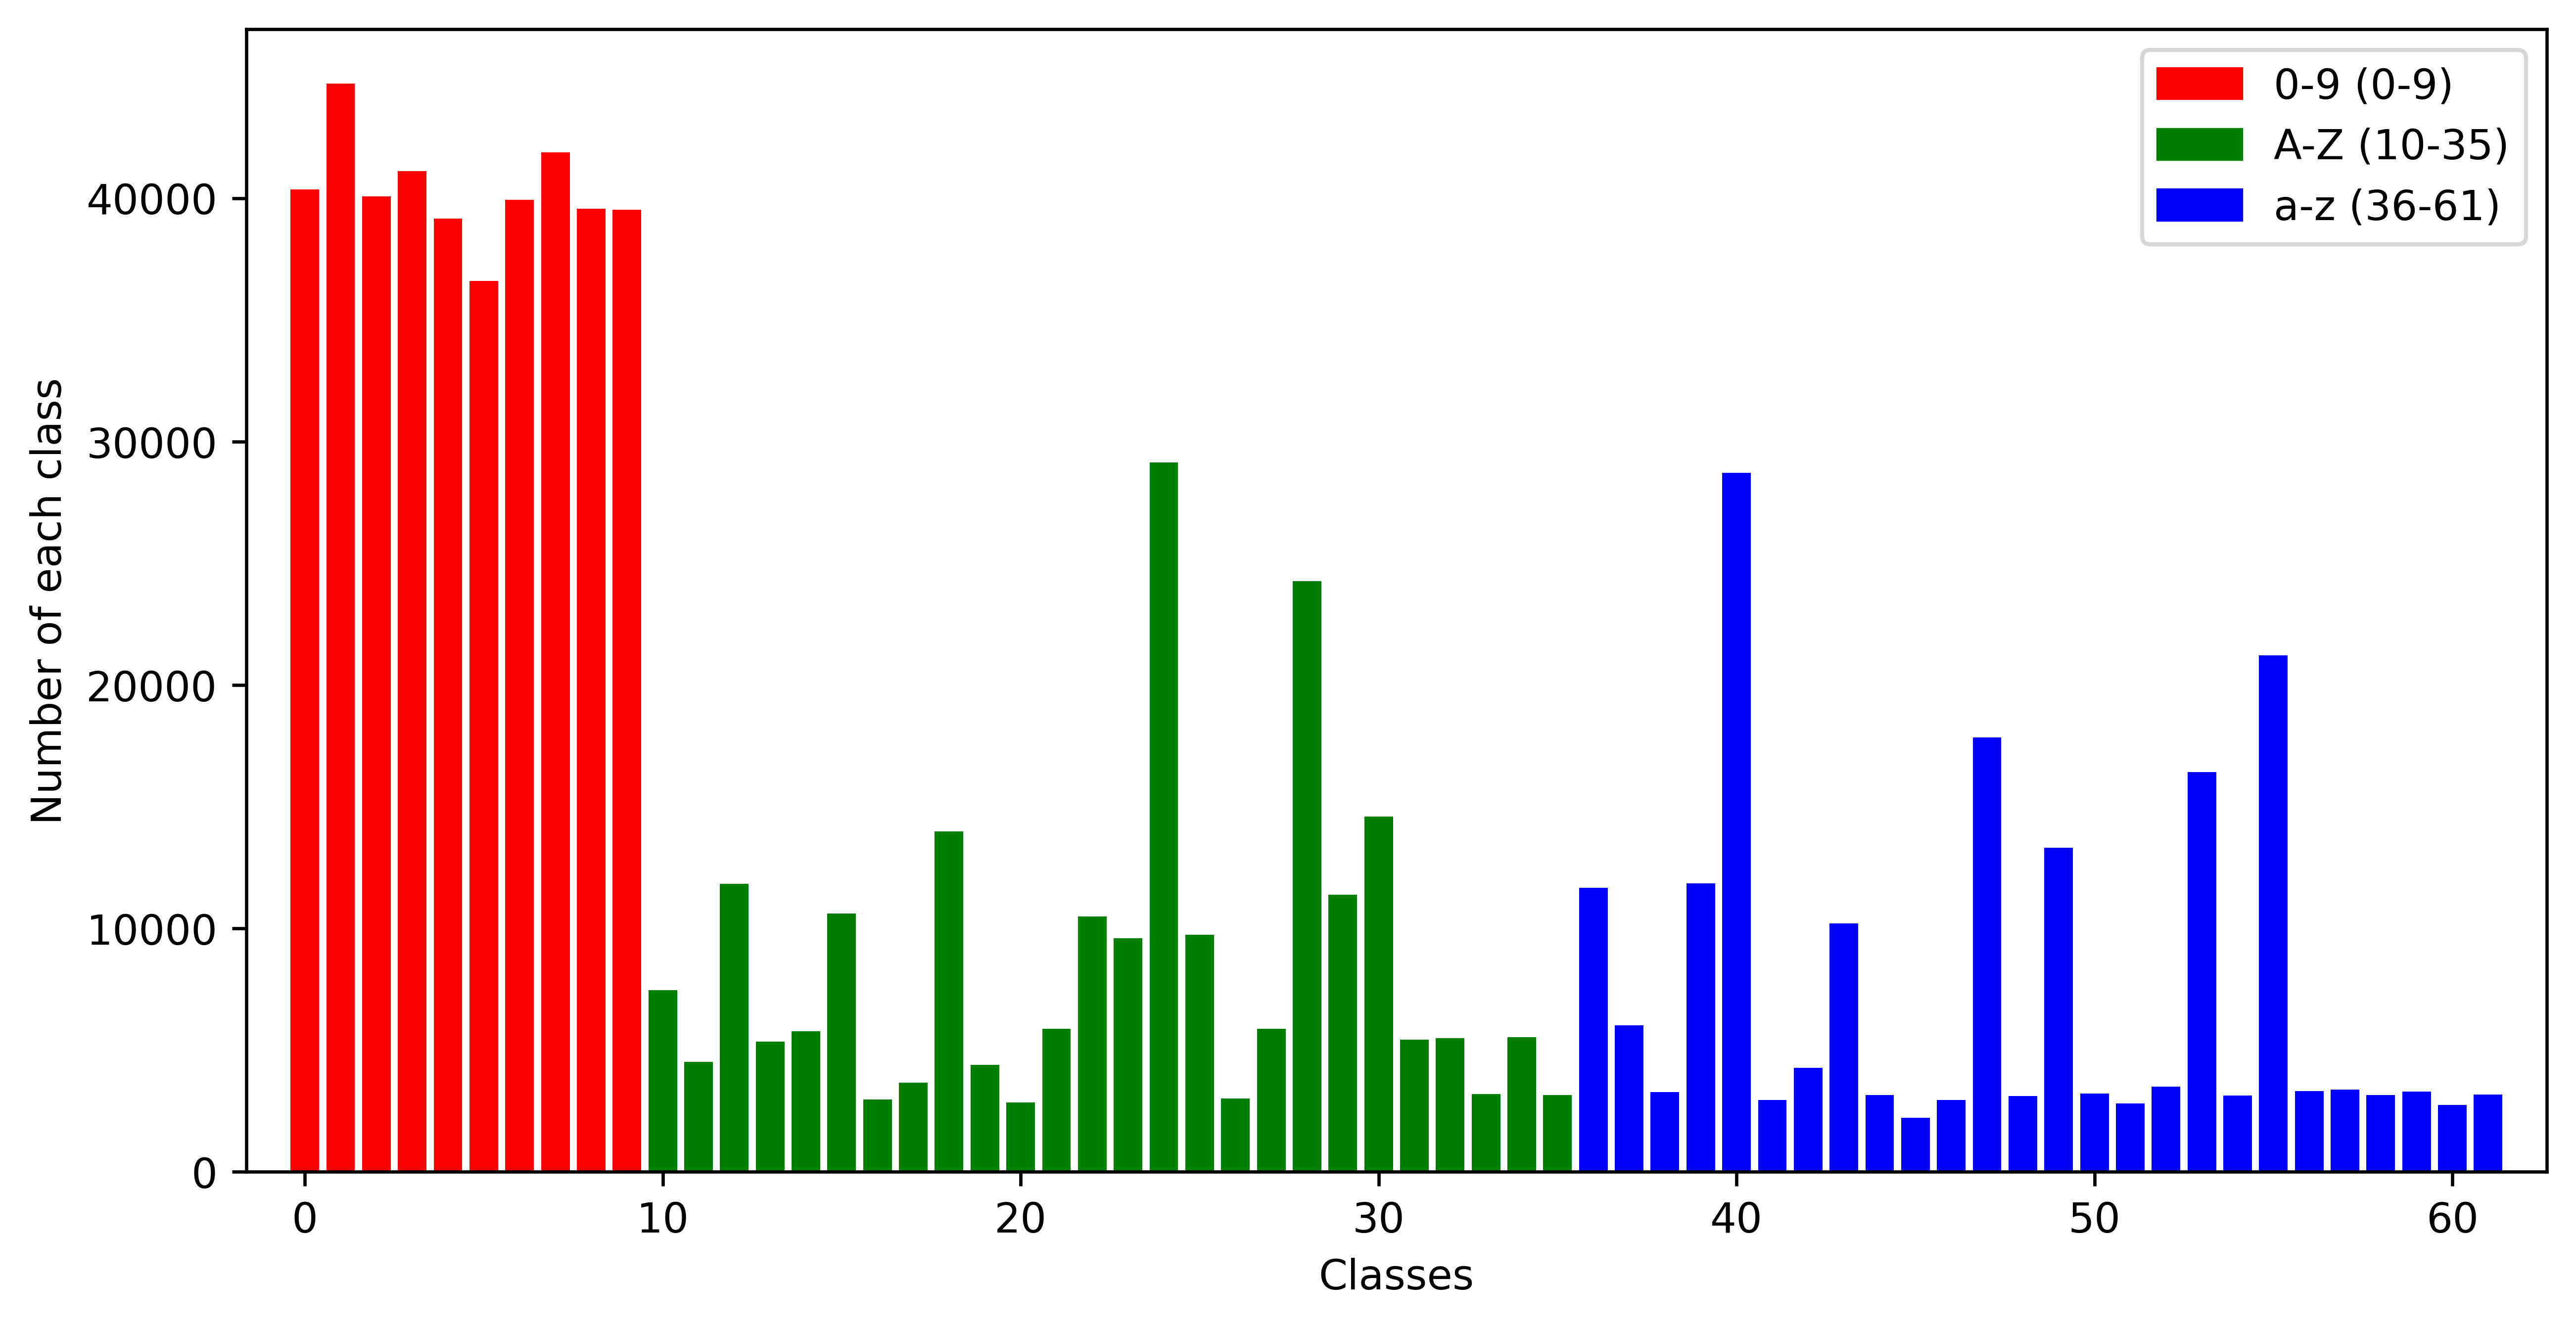
\includegraphics[scale=0.7]{images/chap5/count_all_classes.png}%
	\caption{%
		تعداد داده‌های هر کلاس و نحوه نام‌گذاری در مجموعه داده
		\lr{FEMNIST}.
	}
	\label{count_all_classes}
	\centering
\end{figure}

همان‌طور که در شکل
\ref{count_all_classes}
مشاهده می‌شود، تعداد کلاس‌های 0 تا 9 که به ارقام 0 تا 9 اشاره دارند، به‌طور قابل‌توجهی بیشتر از سایر کلاس‌هاست و هر کدام حدود 40٬000 نمونه دارند. در بین کلاس‌های 10 تا 35 که مربوط به حروف بزرگ انگلیسی هستند، کلاس‌های \lr{S} و \lr{O} بیشترین تعداد نمونه را دارند. به نظر می‌رسد این سبک از جمع‌آوری داده به دلیل جلوگیری از اشتباه گرفتن کلاس \lr{O} با عدد صفر و کلاس \lr{S} با معادل حرف کوچک آن در کلاس‌های 36 تا 61 بوده باشد.


مجموعه داده
\lr{FEMNIST}
به‌صورت پیش‌فرض شامل 3597 کاربر است که داده‌ها میان این کاربران توزیع شده‌اند. این توزیع، نه از لحاظ تعداد تصاویر بین کاربران و نه از لحاظ پوشش‌دهی کلاس‌ها در هر کاربر، یکسان نیست. با این حال، تعداد کاربران و نحوه توزیع داده‌ها میان آن‌ها را می‌توان به دلخواه تغییر داد.



اکنون رویکردهای پایه در مجموعه داده
\lr{FEMNIST}
بررسی خواهند شد. در رویکرد اول، داده‌ها بدون توجه به کاربران اصلی و تنها بر اساس کلاس‌های آن‌ها تفکیک می‌شوند. به این صورت که تمام داده‌های مربوط به هر کلاس جمع‌آوری شده و طبق یک توزیع مشخص بین تعدادی کاربر تقسیم می‌شوند. این روش به عنوان رویکرد کلاس‌بندی یا
\lr{FEMNISTclass}
شناخته می‌شود.

در رویکرد دوم، ساختار اصلی مجموعه داده تغییر نمی‌کند و تعداد کاربران همان تعداد پیش‌فرض باقی می‌ماند. همچنین داده‌ها دقیقا به همان شیوه‌ای که به هر کاربر اختصاص داده شده‌اند، حفظ می‌شوند. این روش به نام رویکرد نویسندگان یا
\lr{FEMNISTwriter}
نام‌گذاری شده است. در ادامه نتایج مربوط به هر کدام از این رویکرد‌ها به‌صورت مجزا بررسی خواهد شد.






\subsubsection{
	مقایسه نتایج در رویکرد کلاس‌بندی
	\lr{\texttt{\fontspec{Times New Roman} (FEMNISTclass)}}
}

نتایج مقایسه روش
\lr{SimFedSwap}
با دیگر روش‌های مرجع در شکل
\ref{result_FEMNISTclass}
نمایش داده شده‌اند که این آزمایش بر روی مجموعه داده
\lr{FEMNISTclass}
انجام شده است. پارامترهای مورد استفاده در این آزمایش نیز در جدول
\ref{tabel_parameter_FEMNISTclass}
ذکر شده‌اند.


\begin{figure}[t]
	\centering
	\subfigure[
	دید کلی از نتیجه
	\qquad\hspace{3mm}]{
		\label{result_FEMNISTclass_base}
		\includegraphics*[width=.48\textwidth]{images/chap5/result/FEMNISTclass/acc_base.png}
	}
	\hspace{0.8mm}
	\subfigure[
	بزرگ‌نمایی شده بخش اصلی					
	\qquad\hspace{5mm}]{
		\label{result_FEMNISTclass_zoom}
		\includegraphics*[width=.48\textwidth]{images/chap5/result/FEMNISTclass/acc_zoom.png}
	}
	\caption{
		مقایسه منحنی‌های دقت در مجموعه داده
		\lr{FEMNISTclass}.
	}
	\label{result_FEMNISTclass}
\end{figure}


%\addtolength{\tabcolsep}{-0.5mm}
\begin{table}[t]
	\centering
	\caption{
		پارامترهای اجرا در مجموعه داده
		\lr{FEMNISTclass}
	}
	\label{tabel_parameter_FEMNISTclass}
	%	\scalebox{0.985}{
		\begin{tabular}{ccccccccccccc}
			\hline
			\specialcell{مجموعه\\داده} &
			\specialcell{شبکه\\عصبی} &
			\specialcell{نحوه\\جابه‌جایی} &
			\specialcell{توزیع\\داده} &
			$K$ &
			$B$ &
			$C$ &
			$SP$ &
			$\eta$ &
			$E$ &
			$h_1$ &
			$h_2$
			\\
			\hline
			\lr{FEMNISTclass} &
			\lr{Conv} &
			\lr{MSS} &
			یکنواخت &
			\lr{200} &
			\lr{1024} &
			\lr{1.0} &
			\lr{1.0} &
			\lr{0.001} &
			\lr{2} &
			\lr{5} &
			\lr{3}
			\\
		\end{tabular}
		%	}
\end{table}



از شکل
\ref{result_FEMNISTclass}
مشخص است که روش‌های مبتنی‌بر جابه‌جایی در مقایسه با
\lr{FedAvg}
عملکرد متفاوتی نشان می‌دهند، اما همچنان تفاوت‌های عملکردی بین آن‌ها محدود و نزدیک به هم است.
نکته قابل توجه این است که بسیاری از تغییرات در نمودارها به لحظات جابه‌جایی یا میانگین‌گیری مربوط می‌شوند.
برای جزئیات بیشتر و بررسی دقیق‌تر، می‌توان به منحنی‌های خطا که در شکل
\ref{app_result_FEMNISTclass}
پیوست آمده‌اند، مراجعه کرد.




\subsubsection{
	مقایسه نتایج در رویکرد نویسندگان
	\lr{\texttt{\fontspec{Times New Roman} (FEMNISTwriter)}}
}
نتایج مربوط به مقایسه روش
\lr{SimFedSwap}
با سایر روش‌های مرجع در شکل
\ref{result_FEMNISTwriter_one}
قابل مشاهده است. این آزمایش بر روی مجموعه داده
\lr{FEMNISTwriter}
اجرا شده و پارامترهای به‌کاررفته در آن نیز در جدول
\ref{tabel_parameter_FEMNISTwriter}
ذکر شده‌اند.


\begin{figure}[t]
	\centering
	\subfigure[
	دید کلی از نتیجه
	\qquad\hspace{3mm}]{
		\label{result_FEMNISTwriter_one_base}
		\includegraphics*[width=.48\textwidth]{images/chap5/result/FEMNISTwriter/acc_base_one.png}
	}
	\hspace{0.8mm}
	\subfigure[
	بزرگ‌نمایی شده بخش اصلی					
	\qquad\hspace{5mm}]{
		\label{result_FEMNISTwriter_one_zoom}
		\includegraphics*[width=.48\textwidth]{images/chap5/result/FEMNISTwriter/acc_zoom_one.png}
	}
	\caption{
		مقایسه منحنی‌های دقت در یک اجرا بر روی مجموعه داده
		\lr{FEMNISTwriter}.
	}
	\label{result_FEMNISTwriter_one}
\end{figure}


%\addtolength{\tabcolsep}{-0.5mm}
\begin{table}[t]
	\centering
	\caption{
		پارامترهای اجرا در مجموعه داده
		\lr{FEMNISTwriter}
	}
	\label{tabel_parameter_FEMNISTwriter}
	%	\scalebox{0.985}{
		\begin{tabular}{ccccccccccccc}
			\hline
			\specialcell{مجموعه\\داده} &
			\specialcell{شبکه\\عصبی} &
			\specialcell{نحوه\\جابه‌جایی} &
			\specialcell{توزیع\\داده} &
			$K$ &
			$B$ &
			$C$ &
			$SP$ &
			$\eta$ &
			$E$ &
			$h_1$ &
			$h_2$
			\\
			\hline
			\lr{FEMNISTwriter} &
			\lr{Conv} &
			\lr{MSS} &
			یکنواخت &
			\lr{3597} &
			\lr{64} &
			\lr{0.15} &
			\lr{1.0} &
			\lr{0.001} &
			\lr{1} &
			\lr{5} &
			\lr{3}
			\\
		\end{tabular}
		%	}
\end{table}


در شکل
\ref{result_FEMNISTwriter_one}
مشاهده می‌شود که روش‌های مبتنی‌بر جابه‌جایی نتایجی متفاوت از روش
\lr{FedAvg}
ارائه داده‌اند. اما نکته مهم، برتری قابل توجه روش‌های مبتنی‌بر شباهت نسبت به
\lr{FedSwap}
است. این اولین آزمایشی است که در آن روش‌های شباهت محور توانسته‌اند عملکرد بهتری را به‌طور معناداری ارائه کنند. برای اطلاعات بیشتر و تحلیل دقیق‌تر، می‌توان به منحنی‌های خطا در شکل
\ref{app_result_FEMNISTwriter_one}
پیوست، مراجعه کرد.



با بهبود نتایج، این پرسش پیش می‌آید که آیا این برتری در شرایط استفاده از چندین
\lr{Seed}
متفاوت، همچنان پابرجا خواهد بود. برای پاسخ به این سوال، آزمایش قبلی با پنج
\lr{Seed}
مختلف تکرار شده و میانگین نتایج در شکل
\ref{result_FEMNISTwriter_seed}
نمایش داده شده‌اند. نکته قابل توجه این است که اختلاف روش مبتنی‌بر شباهت با روش
\lr{FedSwap}%
، دیگر به وضوح قبلی دیده نمی‌شود و تنها، بهبودی حدود یک درصد در میانگین پنج اجرا مشاهده می‌شود.
\begin{figure}[t]
	\centering
	\subfigure[
	دید کلی از نتیجه
	\qquad\hspace{3mm}]{
		\label{result_FEMNISTwriter_seed_base}
		\includegraphics*[width=.48\textwidth]{images/chap5/result/FEMNISTwriter/acc_base_seed.png}
	}
	\hspace{0.8mm}
	\subfigure[
	بزرگ‌نمایی شده بخش اصلی					
	\qquad\hspace{5mm}]{
		\label{result_FEMNISTwriter_seed_zoom}
		\includegraphics*[width=.48\textwidth]{images/chap5/result/FEMNISTwriter/acc_zoom_seed.png}
	}
	\caption{
		مقایسه منحنی‌های دقت در میانگین پنج اجرا بر روی مجموعه داده
		\lr{FEMNISTwriter}.
	}
	\label{result_FEMNISTwriter_seed}
\end{figure}
همچنین باید به این نکته توجه شود که تغییر
\lr{Seed}
در نمودارهای پیشین، تفاوت چشم‌گیری در خروجی ایجاد نمی‌کردند.
برای بررسی جزئیات بیشتر، منحنی‌های خطا در شکل
\ref{app_result_FEMNISTwriter_seed}
پیوست ارائه شده‌اند.


بنابراین می‌توان نتیجه گرفت که با افزایش تعداد کاربران و داده‌های مربوط به آن‌ها، روش‌های مبتنی بر شباهت، هرچند به میزان کم، می‌توانند عملکرد بهتری نشان دهند.
باید به این نکته توجه داشت که دقت کلی که در این مجموعه داده به 50 درصد رسید، وابسته به طراحی شبکه عصبی است. با بهینه‌سازی این شبکه، می‌توان به دقت بالاتری دست یافت. با این حال، این بهینه‌سازی تأثیری بر مقایسه بین روش‌ها نخواهد داشت، زیرا همه روش‌ها به‌طور همزمان به دقت بهتری دست خواهند یافت.



\subsection{
	مقایسه جابه‌جایی حریصانه با جابه‌جایی حداقل شباهت در روش
	\lr{\texttt{\fontspec{Times New Roman} SimFedSwap}}
}

شکل
\ref{result_MSS_vs_GS_FEMNISTwriter}
عملکرد دو روش جابه‌جایی حریصانه و جابه‌جایی حداقل شباهت را در الگوریتم
\lr{SimFedSwap}
مقایسه می‌کند. این آزمایش بر روی مجموعه داده
\lr{FEMNISTwriter}
انجام شده و پارامترهای مربوط به این بررسی در جدول
\ref{tabel_parameter_FEMNISTwriter}
آورده شده است.


\begin{figure}[t]
	\centering
	\subfigure[
	دید کلی از نتیجه
	\qquad\hspace{3mm}]{
		\label{result_MSS_vs_GS_FEMNISTwriter_base}
		\includegraphics*[width=.48\textwidth]{images/chap5/result_MSS_vs_GS/FEMNISTwriter/acc_base.png}
	}
	\hspace{0.8mm}
	\subfigure[
	بزرگ‌نمایی شده بخش اصلی					
	\qquad\hspace{5mm}]{
		\label{result_MSS_vs_GS_FEMNISTwriter_zoom}
		\includegraphics*[width=.48\textwidth]{images/chap5/result_MSS_vs_GS/FEMNISTwriter/acc_zoom.png}
	}
	\caption{
		مقایسه منحنی‌های دقت بین
		\lr{MSS}
		و
		\lr{GS}%
		، در مجموعه داده
		\lr{FEMNISTwriter}.
	}
	\label{result_MSS_vs_GS_FEMNISTwriter}
\end{figure}



نتایج به دست آمده از شکل
\ref{result_MSS_vs_GS_FEMNISTwriter}
نشان می‌دهد که معیار
\lr{OSAD}
با استفاده از جابه‌جایی حریصانه عملکردی مشابه روش
\lr{FedSwap}
داشته است. اما روش‌های
\lr{CKA}
با استفاده از هسته‌های خطی و گاوسی به تدریج عملکرد خود را بهبود بخشیده و به نتایج بهتری دست یافته‌اند. برای اطلاعات دقیق‌تر، منحنی‌های خطا در شکل
\ref{app_result_MSS_vs_GS_FEMNISTwriter}
پیوست، قابل بررسی هستند.




\section{نتیجه‌گیری}

در دنیای امروزی با رشد سریع فناوری و افزایش تعداد دستگاه‌های متصل به اینترنت، نیاز به برقراری ارتباطات مؤثر و حفاظت از حریم شخصی کاربران بیش از پیش اهمیت یافته است. این مسئله منجر به توسعه روش‌های توزیع‌شده‌ای مانند یادگیری فدرال شده است. در یادگیری فدرال، داده‌ها به‌جای ارسال به یک سرور مرکزی برای پردازش، در محل خود دستگاه‌ها نگهداری می‌شوند و مدل‌ها به‌صورت محلی آموزش داده می‌شوند. سپس این مدل‌ها با یکدیگر ترکیب می‌شوند تا یک مدل سراسری به‌دست آید. این روش علاوه بر کاهش نیاز به انتقال داده‌ها، حریم شخصی کاربران را نیز بهتر حفظ می‌کند.

با این حال، یادگیری فدرال با چالش‌های متعددی مواجه است. یکی از این چالش‌ها، ناهمگنی آماری داده‌ها است. به این معناست که داده‌های موجود در دستگاه‌های مختلف می‌توانند بسیار متفاوت و گوناگون باشند. این ناهمگنی باعث می‌شود که مدل‌های محلی نتوانند به‌طور کامل ویژگی‌های تمامی داده‌ها را یاد بگیرند و در نتیجه، مدل سراسری نیز به‌خوبی همگرا نشود. در این شرایط، رسیدن به یک مدل سراسری که عملکرد قابل قبولی داشته باشد، ممکن است با مشکل مواجه شود.

برای مقابله با این چالش، یکی از راهکارهای پیشنهادی، جابه‌جایی وزن‌های شبکه عصبی بین کاربران در طول فرآیند یادگیری است. این روش باعث می‌شود که مدل‌های محلی با داده‌های متنوع‌تری روبه‌رو شوند و در نتیجه، مدل سراسری بتواند به یک همگرایی بهتر دست یابد. به عبارت دیگر، با جابه‌جایی وزن‌ها، مدل‌ها به داده‌های بیشتری دسترسی پیدا می‌کنند که این امر به بهبود کیفیت یادگیری و همگرایی مدل کمک می‌کند.

در روش‌های متداول، جابه‌جایی وزن‌ها به‌طور تصادفی انجام می‌شود، اما در این پژوهش پیشنهاد گردید که به‌جای استفاده از روش تصادفی، این جابه‌جایی به‌صورت هوشمندانه و بر اساس معیارهای شباهت انجام شود، به این صورت که مدل‌هایی که کمترین میزان شباهت را با یکدیگر دارند، جابه‌جا شوند. این رویکرد باعث می‌شود که مدل‌ها با داده‌هایی که به‌طور کامل با آن‌ها آشنا نیستند، روبه‌رو شوند و این امر می‌تواند به بهبود همگرایی مدل سراسری منجر شود. به‌عبارت دیگر، این نوع جابه‌جایی هوشمندانه می‌تواند مدل سراسری را سریع‌تر و بهتر به همگرایی نهایی هدایت کند.

یکی از دستاوردهای جانبی این پژوهش، بررسی تأثیر جابه‌جایی وزن‌ها بر حفظ حریم شخصی کاربران بود. روش‌های مرسوم جابه‌جایی، این فرآیند را به‌طور مستقیم بین کاربران نهایی انجام می‌دهند. این روش اگرچه می‌تواند به کاهش سربار شبکه کمک کند، اما ممکن است به تشدید مشکلات حریم شخصی منجر شود. در این پژوهش، پیشنهاد شد که سرور مرکزی به عنوان واسطه در فرآیند جابه‌جایی عمل کند. با این کار، حریم شخصی کاربران بهتر حفظ می‌شود و پیاده‌سازی روش‌هایی مانند حفظ حریم خصوصی تفاضلی نیز ساده‌تر می‌شد.

%زمینه ساز بهبود در حریم شخصی است اما

باید توجه داشت که هرچند این روش زمینه‌ساز بهبود در حفظ حریم شخصی می‌باشد، اما نسبت به روش‌های جابه‌جایی وزن‌ها بدون دخالت سرور، اندکی به سربار شبکه می‌افزاید. با این حال، این سربار در مقایسه با روش‌های سنتی مانند میانگین‌گیری فدرال همچنان بسیار کمتر خواهد بود. در واقع، مزایایی که این روش در بهبود همگرایی و حفاظت از حریم شخصی به ارمغان می‌آورد، می‌تواند افزایش جزئی سربار شبکه را نسبت به روش‌های جابه‌جایی بدون دخالت سرور توجیه نموده و آن را به یک گزینه مطلوب و کارآمد تبدیل کند.
البته دوباره تاکید می‌شود که حفظ حریم شخصی از اصول کلیدی در یادگیری فدرال به شمار می‌آید و برای ارزیابی دقیق میزان نفوذپذیری آن، لازم است روش‌های تخصصی مرتبط به‌صورت جداگانه اجرا و بررسی شوند. اما می‌توان گفت در این پژوهش، با وجود آن که تمرکز بر بهبود دقت مدل نهایی بوده است، در این مسیر، به حریم شخصی نیز توجه شده است.

در نهایت، این پژوهش نشان داد که جابه‌جایی مدل‌های شبکه عصبی به‌صورت هوشمندانه و بر اساس معیارهای شباهت، می‌تواند فرآیند همگرایی مدل سراسری را تسریع کند. این امر به‌ویژه در شرایطی که تعداد کاربران زیاد باشد، اثرات مثبت خود را بهتر نشان می‌دهد. به بیان دیگر، هرچه تعداد کاربران بیشتر باشد، مزایای استفاده از این روش بیشتر خواهد بود و بهبود قابل توجهی در فرآیند همگرایی مشاهده می‌شود.

بنابراین، در مواردی که تعداد کاربران زیاد است و داده‌ها بسیار متفاوت و پراکنده هستند، استفاده از روش‌ جابه‌جایی وزن‌ها بر پایه شباهت می‌تواند بهبود قابل ملاحظه‌ای در کارایی و سرعت همگرایی مدل سراسری به‌همراه داشته باشد. این روش نه‌تنها از نظر فنی مؤثر است، بلکه از دیدگاه حفاظت از حریم شخصی نیز بسیار مناسب به‌نظر می‌رسد.

در نتیجه، این پژوهش اهمیت و تأثیر جابه‌جایی هوشمندانه وزن‌های شبکه‌های عصبی در یادگیری فدرال را برجسته کرد و راهکاری جدید برای بهبود فرآیند همگرایی و حفظ حریم شخصی کاربران ارائه داد. این رویکرد می‌تواند به‌عنوان یک راه‌حل مؤثر در مواجهه با چالش‌های موجود در یادگیری فدرال مورد استفاده قرار گیرد.


